\topheading{CuTe-MCFM}

\includegraphics[width=0.4\textwidth]{./sections/cute-mcfmpic.png}
\midheading{N$^3$LL and N$^4$LL $q_T^2$ resummation for color-singlet processes in MCFM}

Based on \href{https://arxiv.org/abs/2009.11437}{arXiv:2009.11437} (Becher, Neumann '20).

The $q_T$ resummation in CuTe-MCFM is available for color-singlet processes and based on a 
factorization theorem in SCET. It is fully differential in the Born kinematics and matches
to large-$q_T^2$ fixed-order predictions at relative order
$\alpha_s^2$. It provides an efficient way to estimate uncertainties from
fixed-order truncation, resummation, and parton distribution
functions. In addition to $W, Z$ and $H$ production, also the diboson
processes $\gamma\gamma$, $Z\gamma$, $ZH$, $WH$, $WW$, $WZ$ and $ZZ$ are available, including decays.

While CuTe-MCFM can calculate $q_T$-resummed results without using
pregenerated beam functions grids, we recommend that LHAPDF grid files are
generated for the beam functions beforehand for a choice of a PDF set. This
\emph{significantly} accelerates the evaluation of the beam functions and the
integration.

CuTe-MCFM ships with pregenerated beamfunction grids for the central
values of \texttt{CT14nnlo} and \texttt{NNPDF31\_nnlo\_as\_0118}, which
are included in the \texttt{Bin/PDFs} directory. This path is automatically used
as the preferred path for LHAPDF grid files. With these pregenerated
grids the example input files work out of the box. For other PDF sets or
when using PDF errors, the first run of CuTe-MCFM should be with the
setting \texttt{makegrid=.true.}. Additionally the input and output
directories for the PDF grids have to be specified. For example the
input directory is typically \texttt{/usr/local/share/LHAPDF/} (or the
\texttt{PDFs/} directory relative to the mcfm executable in \texttt{Bin}) and
the output directory should be a user-writeable directory like
\texttt{/home/user/gridout/} (or \texttt{PDFs/}). Note the trailing slashes.

When calling mcfm with \texttt{makegrid=.true.} only the beam function
grids are written during that run, and mcfm exits afterwards.
We recommend to use \texttt{PDFs/} as the gridout path, since this
path is automatically added to the LHAPDF search paths, and you won't have to
copy the generated grid directories to your LHAPDF grid directory or set the
\texttt{LHAPDF\_DATA\_PATH} environment variable to the gridout path.

For example for the set CT14nnlo the grid directories
\texttt{CT14nnlo\_B00}, \texttt{CT14nnlo\_B10}, \texttt{CT14nnlo\_B11},
\texttt{CT14nnlo\_B20}, \texttt{CT14nnlo\_B21}, \texttt{CT14nnlo\_B22} and \texttt{CT14nnlo\_G10} 
are written and have to be copied to the
directory where LHAPDF searches for the grid files. When the gridout path is chosen as 
\texttt{PDFs/} no further action is necessary. The LHAPDF grid file
search path can be modified by setting the shell
environment variable \texttt{LHAPDF\_DATA\_PATH} to the desired
directory, but the \texttt{PDFs} directory is always used as the preferred directory.


The next run of mcfm should be done with \texttt{makegrid=.false.} and \texttt{usegrid=.true.}.

Other important parameters for the resummation are \texttt{res\_range},
determining the integration range of the purely resummed part,
\texttt{resexp\_range}, determining the integration range of the
fixed-order expanded resummed part, and \texttt{fo\_cutoff} which sets
the lower $q_T$ cutoff for the fixed-order part. Typically this cutoff
should agree with the lower range of \texttt{resexp\_range}. For example
for $Z$ production one can integrate up to $m_Z$ with a cutoff of 1 GeV: \texttt{res\_range = 
0.0 90.0},
\texttt{resexp\_range = 1.0 90.0}, \texttt{qt\_cutoff = 1.0}.

For details regarding these parameters see the next section. The
transition function is also discussed below.

\hypertarget{input-file-parameters}{%
	\midheading{Input file parameters}\label{input-file-parameters}}

The \texttt{[resummation]} section has been added to the input file to
control the resummation. The following keys are available:

\begin{longtable}[]{@{}ll@{}}
%	\toprule
	\begin{minipage}[b]{0.24\columnwidth}\raggedright
		Key\strut
	\end{minipage} & \begin{minipage}[b]{0.71\columnwidth}\raggedright
		Description\strut
	\end{minipage}\tabularnewline
%	\midrule
	\endhead
	\begin{minipage}[t]{0.24\columnwidth}\raggedright
		\texttt{usegrid}\strut
	\end{minipage} & \begin{minipage}[t]{0.71\columnwidth}\raggedright
		\texttt{.true.} or \texttt{.false.} determines whether pregenerated
		LHAPDF interpolation grids should be used for the resummation beam
		functions.\strut
	\end{minipage}\tabularnewline
	\begin{minipage}[t]{0.24\columnwidth}\raggedright
		\texttt{makegrid}\strut
	\end{minipage} & \begin{minipage}[t]{0.71\columnwidth}\raggedright
		If \texttt{.true.}, then MCFM runs in grid generation mode. This
		generates LHAPDF grid files in the directory \texttt{gridoutpath} from
		LHAPDF grids in the directory \texttt{gridinpath}. After the grid
		generation MCFM stops and should be run subsequently with
		\texttt{makegrid = .false.} and \texttt{usegrid = .true.}. When
		\texttt{lhapdf\%dopdferrors=.true.} then also grids for the error sets
		are generated.\strut
	\end{minipage}\tabularnewline
	\begin{minipage}[t]{0.24\columnwidth}\raggedright
		\texttt{gridoutpath}\strut
	\end{minipage} & \begin{minipage}[t]{0.71\columnwidth}\raggedright
		Output directory for LHAPDF grid files, for example
		\texttt{/home/tobias/local/share/LHAPDF/}\strut
	\end{minipage}\tabularnewline
	\begin{minipage}[t]{0.24\columnwidth}\raggedright
		\texttt{gridinpath}\strut
	\end{minipage} & \begin{minipage}[t]{0.71\columnwidth}\raggedright
		Input directory for LHAPDF grid files, for example
		\texttt{/home/tobias/local/share/LHAPDF/}\strut
	\end{minipage}\tabularnewline
	\begin{minipage}[t]{0.24\columnwidth}\raggedright
		\texttt{res\_range}\strut
	\end{minipage} & \begin{minipage}[t]{0.71\columnwidth}\raggedright
		Integration range of purely resummed part, for example \texttt{0.0 80.0}
		for $q_T$ integration between 0 and 80 GeV.\strut
	\end{minipage}\tabularnewline
	\begin{minipage}[t]{0.24\columnwidth}\raggedright
		\texttt{resexp\_range}\strut
	\end{minipage} & \begin{minipage}[t]{0.71\columnwidth}\raggedright
		Integration range of fixed-order expanded resummed part, for example
		\texttt{1.0 80.0} for $q_T$ integration between 1 and 80 GeV.\strut
	\end{minipage}\tabularnewline
	\begin{minipage}[t]{0.24\columnwidth}\raggedright
		\texttt{fo\_cutoff}\strut
	\end{minipage} & \begin{minipage}[t]{0.71\columnwidth}\raggedright
		Lower $q_T$ cutoff $q_0$ for the fixed-order part, see eq.~\eqref{eq:matchingmod} below. 
		Typically the value should agree with the lower range of \texttt{resexp\_range}.\strut
	\end{minipage}\tabularnewline
	\begin{minipage}[t]{0.24\columnwidth}\raggedright
		\texttt{transitionswitch}\strut
	\end{minipage} & \begin{minipage}[t]{0.71\columnwidth}\raggedright
		Parameter passed to the plotting routine to modify the transition
		function, see text.\strut
	\end{minipage}\tabularnewline
%	\bottomrule
\end{longtable}

We strongly recommend to calculate resummed results with pregenerated
grids, see the previous section.
The integration range for the purely resummed part can be controlled with the key
\texttt{res\_range} and should typically be between $0$ and some upper
value. For example for $W^\pm, Z$ or $H$ production this can just be
the boson mass. For other processes there can be thresholds and this
number must be selected more carefully to not run into numerical issues,
see arXiv:2009.11437.

The setting \texttt{resexp\_range} and \texttt{fo\_cutoff} are relevant
for the matching corrections. The values of the \texttt{resexp\_range}
determine the integration range for the fixed-order expansion of the
resummed part. The minimum should typically be at least one GeV for
numerical stability. For smaller values significantly more time goes
into the integration, and the minimum number of Vegas calls might need
to increased. For single boson processes the maximum value can again be
the boson mass, although it can be set to a value where the implemented
transition function fully switches to zero. The fixed-order cutoff
\texttt{fo\_cutoff} determines the minimum $q_T$ for the fixed-order
calculation. This should typically agree with the lower range of the
\texttt{resexp\_range}.

Lastly, the parameter \texttt{transitionswitch} is passed for
convenience to the plotting routines where the transition function is
implemented. It can be used for for an easy control of the transition
region as described in the following.

\hypertarget{plotting-and-transition}{%
	\midheading{Plotting routine and transition function}\label{plotting-and-transition}}

The following transition function is implemented for the example
input files. For more details we refer to our publication. The fully
matched cross-section is described in general by 

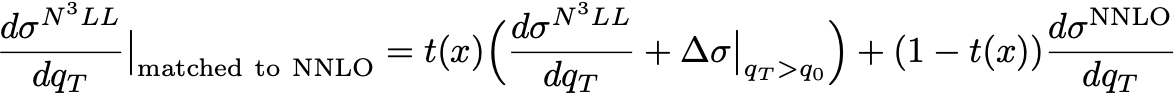
\includegraphics[width=0.9\textwidth]{./sections/Matching.png}
%\begin{equation}\label{eq:matchingmod}
%        \;
%	\left.\frac{\mathrm{d}\sigma^{\text{N$^3$LL}}}{\mathrm{d}q_T}\right|_{\text{matched to \NNLO{}}} 
%	=  t(x) \left( \frac{\mathrm{d}\sigma^{\text{N$^3$LL}}}{\mathrm{d}q_T} + 
%	\left.\Delta\sigma\right|_{q_T>q_0} \right)
%	+ (1-t(x)) \frac{\mathrm{d}\sigma^\NNLO{}}{\mathrm{d}q_T}\,
%\end{equation}

using a transition function $t(x)$. We have implemented a transition function $t$
with $x=q_T^2/Q^2$ that smoothly switches between 1 and 0 like a sigmoid function.

Following a choice in CuTe, we first define

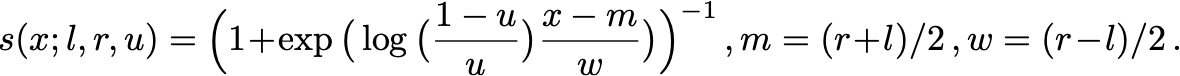
\includegraphics[width=0.9\textwidth]{./sections/sfunction.png}
%\begin{equation}
%s(x;l,r,u) = \left (1 + \exp\left(\log\left(\frac{1-u}{u}\right) \frac{x-m}{w}\right) \right )^{-1}\,,\quad
%m = (r+l)/2\,,\quad w = (r-l)/2\,.
%\end{equation}

The function $s(x)$, parametrized by $l,r,u$, is defined to be $s(l)=1-u$ and $s(r)=u$.
In terms of this sigmoid, our transition function $t(x; x^{\text{min}},x^{\text{max}},u)$, where 
$x=q_T^2/Q^2$, is then defined by
\begin{equation}\label{eq:transition}
	t(x; x^{\text{min}},x^{\text{max}},u) = \left\{\begin{array}{lr}
		1 , & \text{for } x < x^{\text{min}}\\
		\frac{s(x; x^{\text{min}}, x^{\text{max}},u)}
		     {s(x^{\text{min}}; x^{\text{min}}, x^{\text{max}},u)}, & 
		\text{otherwise}
	\end{array}\right\}\,.
\end{equation}
This ensures that below $x^{\text{min}}=(q_T^{\text{min}}/Q)^2$ only the naively matched result is 
used, and at
$x^{\text{max}}$
for small $u\ll1$ the transition function is approximately $u$. In practice it makes sense to set 
the transition
function to zero below a small threshold like $10^{-3}$ without a noticeable discontinuity.
This has the advantage that the deteriorating resummation and matching corrections do not impact 
the region of 
large $q_T$ at all.
Our example plotting routines use $x^{\text{min}}=0.001$, and $u=0.001$, and the parameter 
$x^{\text{max}}$ corresponds to the value of \texttt{transitionswitch} set in the input file. The 
transition function can be changed or completely replaced by just modifying the plotting routines. 
The following figure illustrates this transition function.

\begin{figure}[t!]
	\centering
	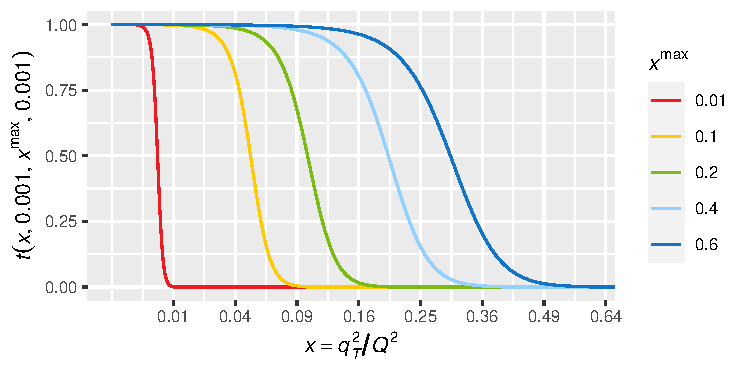
\includegraphics[width=0.8\textwidth]{transition.pdf}
	\caption{The transition function defined in eq.~\eqref{eq:transition} for different values of 
	the parameter $x^{\text{max}}$ which determines the position of the 
		transition. The $x$-axis is displayed on a square-root scale 
		to guide the eye on 
		the quadratic $q_T$-dependence.}
	\label{fig:transition}
\end{figure}

\midheading{Modifying the plotting routines and transition function.}
The plotting infrastructure has been completely rewritten for CuTe-MCFM, and we recommended to only 
use the new infrastructure
from this point on by setting \texttt{histogram\%newstyle = .true.} in
the input file. This is the default for the CuTe-MCFM example input files.

For the processes $W^\pm,Z,H$, $\gamma\gamma$, $Z\gamma$, $ZH$
and $W^\pm H$ we include predefined plotting routines that can be
adjusted. For example for $Z$ production the plotting routine is in the file
\texttt{src/User/nplotter\_Z\_new.f90}, and similarly for the other processes.
The routine \texttt{setup} defines all histograms with custom or uniform
binning and names. The
number of used histograms needs to be allocated in this routine. The
routine \texttt{book} is called for each phase space point. Through the
boolean variable \texttt{abovecut} it is known whether the routine is
called for ``boosted $q_T=0$'' (resummed part and fixed-order expansion of
resummed part) or for $q_T>0$ (fixed-order). All provided example input files
use the transition function as defined above, see also \href{https://arxiv.org/abs/2009.11437}{arXiv:2009.11437}.

The plotting routine returns the calculated observables in the
\texttt{vals} array, and Vegas weights in \texttt{wts}. The transition
function is implemented by reweighting the original Vegas weights with
the output of the transition function. To disable the transition
function, one sets \texttt{trans} to $1$ before filling the \texttt{wts}
array.

Apart from modifying a default set of kinematical cuts in the input
file, cuts can also be set in the file
\texttt{src/User/gencuts\_user.f90} in a fully flexible way based on the
event's four momenta. Some commented out examples are included there.



